\subsubsection{Reading in compositional initial composition files generated with geomIO}
\label{sec:geomio}
\textit{This section was contributed by Juliane Dannberg}

\note{This cookbook is based on a developer version of geomIO from July 2016. In the meantime, the development of
geomIO continued, and there is now a publication\cite{bauvillegeomio} that describes its features and how they can be used in more detail.}

Many geophysical setups require initial conditions with several different materials and complex geometries.
Hence, sometimes it would be easier to generate the initial geometries of the materials as a drawing instead
of by writing code. The MATLAB-based library geomIO (\url{https://bitbucket.org/geomio/geomio}, \cite{bauvillegeomio}) provides a convenient tool
to convert a drawing generated with the vector graphics editor Inkscape (\url{https://inkscape.org/en/}) to a data
file that can be read into \aspect{}. Here, we will demonstrate how this can be done for a 2D setup for a model
with one compositional field, but geomIO also has the capability to create 3D volumes based on a series of 2D vector
drawings using any number of different materials. Similarly, initial conditions defined in this way can also be used with particles
instead of compositional fields.

To obtain the developer version of geomIO, you can clone the bitbucket repository by executing the command
\begin{verbatim}
 git clone https://bitbucket.org/geomio/geomio.git
\end{verbatim}
or you can download geomIO \href{https://bitbucket.org/geomio/geomio/downloads}{here}.
You will then need to add the geomIO source folders to your MATLAB path by running the file located in
\texttt{/path/to/geomio/installation/InstallGeomIO.m}.
An extensive documentation for how to use geomIO can be found \href{http://geomio-doc.bitbucket.org/}{here}.
Among other things, it explains \href{http://geomio-doc.bitbucket.org/tuto2D.html#drawing}{how to generate drawings in Inkscape}
that can be read in by geomIO, which involves assigning new attributes to paths in Inkscape's XML editor.
In particular, a new property `phase' has to be added to each path, and set to a value corresponding to the
index of the material that should be present in this region in the initial condition of the geodynamic model.

\note{geomIO currently only supports the latest stable version of Inkscape (0.91), and other versions might not
  work with geomIO or cause errors. Moreover, geomIO currently does not support grouping paths (paths can still
  be combined using \texttt{Path$\rightarrow$Union}, \texttt{Path$\rightarrow$Difference} or similar commands),
  and only the outermost closed contour of a path will be considered. This means that, for example, for modeling a spherical
  annulus, you would have to draw two circles, and assign the inner one the same phase as the background of your drawing.}

We will here use a drawing of a jellyfish located in \url{jellyfish.svg}, where different phases
have already been assigned to each path (Figure~\ref{fig:jelly-picture}).
\begin{figure}[tb]
    \centering
    \includesvg[width=0.2\textwidth]{jellyfish.svg}
    \caption{\it Vector drawing of a jellyfish.}
    \label{fig:jelly-picture}
\end{figure}
\note{The page of your drawing in Inkscape should already have the extents (in px) that you later want to use in your model (in m).}

After geomIO is initialized in MATLAB, we \href{http://geomio-doc.bitbucket.org/tuto2D.html#assigning-phase-to-markers}
{run geomIO as described in the documentation}, loading the default options and then specifying all the option we want to
change, such as the path to the input file, or the resolution:
\lstinputlisting[language=matlab]{run_geomio.part1.m}
You can view all of the options available by typing \texttt{opt} in MATLAB.

In the next step we create the grid that is used for the coordinates in the \texttt{ascii data} initial conditions file
and assign a phase to each grid point:
\lstinputlisting[language=matlab]{run_geomio.part2.m}
You can plot the \texttt{Phase} variable in MATLAB to see if the drawing was read in and all phases are assigned correctly
(Figure~\ref{fig:jelly-plot}).
\begin{figure}[tb]
    \centering
    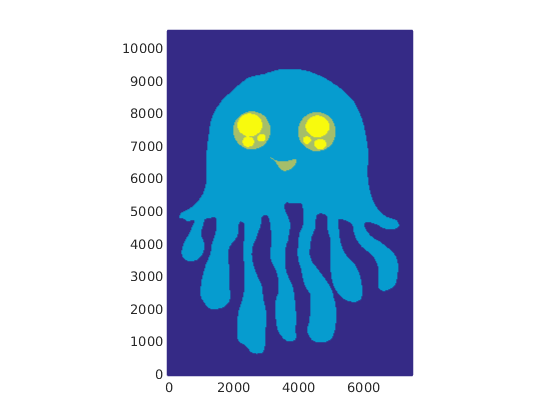
\includegraphics[width=0.45\textwidth]{jelly.png}
    \caption{\it Plot of the \texttt{Phase} variable in MATLAB.}
    \label{fig:jelly-plot}
\end{figure}
Finally, we want to write output in a format that can be read in by \aspect{}'s \texttt{ascii data} compositional
initial conditions plugin. We write the data into the file \texttt{jelly.txt}:
\lstinputlisting[language=matlab]{save_file_as_txt.m}

To read in the file we just created (a copy is located in \aspect{}'s data directory),
we set up a model with a box geometry with the same extents we specified for the drawing in px
and one compositional field. We choose the \texttt{ascii data} compositional initial conditions and specify that we
want to read in our jellyfish. The relevant parts of the input file are listed below:
\lstinputlisting[language=prmfile]{geomIO.prm.out}

If we look at the output in \texttt{ParaView}, we can see our jellyfish, with the mesh refined at the
boundaries between the different phases (Figure~\ref{fig:jelly-paraview}).
\begin{figure}[tb]
    \centering
    \includesvg[width=0.55\textwidth]{jelly-paraview.svg}
    \caption{\it \aspect{} model output of the jellyfish and corresponding mesh in ParaView.}
    \label{fig:jelly-paraview}
\end{figure}

For a geophysical setup, the MATLAB code could be extended to write out the phases into several different columns
of the ASCII data file (corresponding to different compositional fields). This initial conditions file could then be
used in \aspect{} with a material model such as the \texttt{multicomponent} model, assigning each phase different
material properties.

An animation of a model using the jellyfish as initial condition and assigning it a higher viscosity can be found here: \url{https://www.youtube.com/watch?v=YzNTubNG83Q}.


